\documentclass{article}
\usepackage[default]{gillius}
\usepackage{tikz}

\usetikzlibrary{positioning}
\usetikzlibrary{arrows}

\begin{document}
\pagestyle{empty}

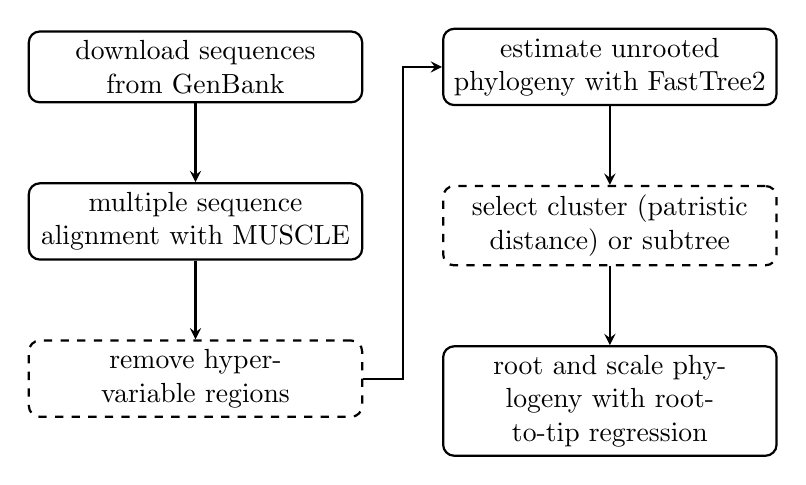
\begin{tikzpicture}
  [every node/.style={rectangle, draw, text width=4cm, align=center, rounded corners},
   every path/.style={->, >=stealth, thick}]
  \node (dl) {download sequences \\ from GenBank};
  \node (align) [below=of dl] {multiple sequence alignment with MUSCLE};
  \node (clip) [below=of align, dashed] {remove hypervariable regions};
  \node (tree) [right=of dl] {estimate unrooted phylogeny with FastTree2};
  \node (cluster) [below=of tree, dashed] {select cluster (patristic distance) or subtree};
  \node (root) [below=of cluster] {root and scale phylogeny with root-to-tip regression};
  
  \draw (dl) -- (align);
  \draw (align) -- (clip);
  \draw (clip.east) -- ++ (0.5cm, 0) |- (tree);
  \draw (tree) -- (cluster);
  \draw (cluster) -- (root);
\end{tikzpicture}

\end{document}
